\documentclass[12pt]{article}

% Rewrite \maketitle command
\makeatletter
\def\thickhrulefill{\leavevmode \leaders \hrule height 1pt\hfill \kern \z@}
\def\maketitle{
    \null \thispagestyle{empty} 
    \vskip 1cm
    \begin{flushright}\normalfont\Large\@author\\\end{flushright}
    \vfil
    \hrule height 2pt
    \par
    \begin{center}\huge \strut \@title \par  
    \begin{scriptsize}(\@date)\end{scriptsize} 
    \end{center}
    \hrule height 2pt
    \begin{center}
\includegraphics[width=0.20\textwidth]{images/hs.png}\end{center}
    \begin{center}\huge Hochschule Ravensburg-Weingarten \\ University of Applied Sciences\end{center}
    \par \vfil \vfil \null
}
\makeatother

% Packages
\usepackage[utf8]{inputenc}  % Encoding
\usepackage[T1]{fontenc}     % Font encoding
\usepackage{graphicx}        % Include graphics
\usepackage{geometry}        % Page layout
\geometry{a4paper, margin=1in} % Set paper size and margins
\usepackage{amsmath}         % Mathematics
\usepackage{lipsum}          % Dummy text
\usepackage{setspace}        % Line spacing control
\setstretch{1.5}             % Equivalent to \linespread{1.5}
\usepackage{hyperref}        % Hyperlinks
\usepackage{listings}        % Listings
\usepackage{caption}         % Captions
\usepackage[justification=centering]{caption}  % This will center all captions


% Add biblatex package with biber as backend
\usepackage[backend=biber, style=numeric, citestyle=numeric]{biblatex}
\addbibresource{literature.bib} % Link to your bibliography file

% Provides command patching capabilities
\usepackage{etoolbox}  
\pretocmd{\section}{\cleardoublepage}{}{}

% Customized header
\usepackage{fancyhdr}
\pagestyle{fancy}
\fancyhf{} % clear all header and footer fields
\renewcommand{\headrulewidth}{0.4pt} % horizontal line under the header

\setlength{\headheight}{15pt} % Change headheight to avoid fancyhdr warnigns

\rhead{\leftmark} % Left header: only title
\renewcommand{\sectionmark}[1]{\markboth{\uppercase{#1}}{}}  % Updates leftmark with only uppercase section title
\cfoot{\thepage} % Center footer: page number

\usepackage{chngcntr}
\counterwithout{table}{section}  % Removes dependency on the section
\counterwithout{table}{subsection}  % Removes dependency on the subsection
  % Include all packages and settings

\begin{document}

% Title page
\title{Seminar Nachhaltigkeit Protokoll: KI für klimaresiliente Städte (Smart Cities)}
\author{Owusu Joseph Kwabena (15542936)\\[1ex]
Volodymyr Kryvytskyi (12042811)\\[1ex]
Supervisor: Prof. Dr. rer. nat. Markus Pfeil}
\date{\today} % or any specific date

\maketitle

% Table of contents
\tableofcontents
\setcounter{page}{1} % Resets page numbering

\section{Abstract}
There is always the constant need to improve civilization and technology, yet this advancement 
often has direct and negative effects on our environment. As we would say in economics, 
we have to make trade-offs. The challenge, therefore, is to find a crucial balance: advancing 
technology and civilization while simultaneously finding sustainable ways to protect our environment, 
especially as urban areas become increasingly vulnerable to climate-related stresses.

This seminar paper explores the frameworks of Artificial Intelligence (AI) for data-oriented 
decision-making for climate-resilient cities (Smart Cities). The analysis focuses on two core 
applications: First, the prediction of extreme weather events (Hitzewellen, Starkregen) using 
advanced AI-driven models based on satellite and real-time sensor data, aimed at establishing 
more accurate and faster early warning systems for public safety. Second, the AI-controlled 
optimization of urban infrastructure, with a specific focus on rainwater management 
to prevent flooding and intelligently manage valuable water resources.

This paper doesn't only details the technical possibilities and advantages of AI in this 
context, but through text-driven analysis of current research, international case studies, 
and expert interviews, how robust and adaptive AI systems can significantly enhance urban 
resilience to climate change. The objective is to evaluate the transformative potential of AI 
in enhancing urban resilience, explaining the evolution of these models, and outlining the necessary 
framework conditions for ecologically, economically, and socially sustainable implementation.
\section{Introduction}
\subsection{Background and Motivation}

The acceleration of climate change is a pressing challenge for global civilization: how to sustain 
technological and economic development while ensuring planetary health. This tension is nowhere more serious 
than in urban environments, which are both foundational elements of human progress and highly vulnerable center 
points for climate risks. Extreme weather events—particularly intense heatwaves, prolonged drought, and 
destructive heavy rainfall—are placing unprecedented stress on urban populations and their foundational 
infrastructure systems. For the records, the effects of climate are already being felt in many cities around the world,
the flood in Germany June 2024 which make the then chancellor Olaf Scholz said that the flooding in the south is a 
reminder that "halting man-made climate change" cannot be neglected \cite{bbc2024germany}. 
For cities to remain habitable and functional, we must evolve from static systems 
into dynamic, "climate-resilient" entities. This necessity provides the core motivation for this paper: 
exploring the role of advanced technology, specifically Artificial Intelligence, in building that resilience.

\subsection{The Resilience}
Climate Resilience in cities means more than just resisting change; it means the ability of the urban system to anticipate, 
absorb, and recover effectively from the negative impacts of climate change.
Traditional urban planning and infrastructure management rely on static modeling and historical averages, 
creating a "resilience gap" when faced with the increasing frequency and unpredictability of extreme weather. 
This gap manifests in two critical areas:

\subsubsection{Reactive Management} The inability to predict and respond to localized micro-climate events in real-time.

\subsubsection{Inefficient Infrastructure} Fixed systems, such as drainage and power grids, cannot adapt dynamically to 
sudden changes in environmental load, leading to damage, energy waste, and public hazard.

Closing this gap requires a swift shift towards data-driven, adaptive cities management (Smart Cities).

\subsubsection{Defining Artificial Intelligence and Machine Learning}

Artificial Intelligence (AI) refers to the capability of computational systems to perform tasks typically associated 
with human intelligence, such as learning, reasoning, and decision-making. Artificial intelligence (AI) is technology that 
enables computers and machines to simulate human learning, comprehension, problem solving, decision making, creativity and autonomy.

Applications and devices equipped with AI can see and identify objects. They can understand and respond to human language. 
They can learn from new information and experience. They can make detailed recommendations to users and experts. They can act 
independently, replacing the need for human intelligence or intervention (a classic example being a self-driving car)\cite{ibmThinkAI}.

The vast majority of modern applications, 
including those discussed here, rely on Machine Learning (ML). ML is the process where algorithms create an AI model—a 
mathematical structure—by identifying complex patterns within large datasets. This process is called training. During training, 
the system is fed vast amounts of data (e.g., historical weather records, sensor readings) and iteratively adjusts its internal 
parameters to minimize prediction errors. This results in a predictive or decision-making system capable of accurate analysis 
and autonomous response.

\subsubsection{History and Evolution of AI and ML}
Since the early 1950s, artificial intelligence (AI) has been an active area of research and development in computer science.
The term “artificial intelligence” was coined in 1956 by John McCarthy\cite{datascientest_mccarthy}, who is widely regarded as the father of AI.
AI systems have been designed to mimic various aspects of human intelligence, including learning, reasoning, problem-solving, 
perception, and language understanding.

In the 1980s, Machine Learning (ML) emerged as a subfield of AI, focusing on the development of algorithms that enable computers 
to learn from data and make predictions or decisions without being explicitly programmed for every task.

In the 2010s, the advent of Deep Learning (DL)—a subset of ML based on artificial neural networks—revolutionized the field by 
enabling the processing of large datasets and achieving unprecedented accuracy in tasks such as image and speech recognition. 
These models are designed to mimic certain aspects of the human brain’s functionality.

More recently, the breakthroughs of the 2020s have given rise to Generative AI models, which refer to deep learning architectures 
capable of creating original and complex content—such as long-form text, high-quality images, realistic video, or audio—in response 
to user prompts.

At a high level, generative models learn from vast amounts of training data to generate new data that share similar characteristics 
with the original examples.

\begin{figure}[h]
    \centering
    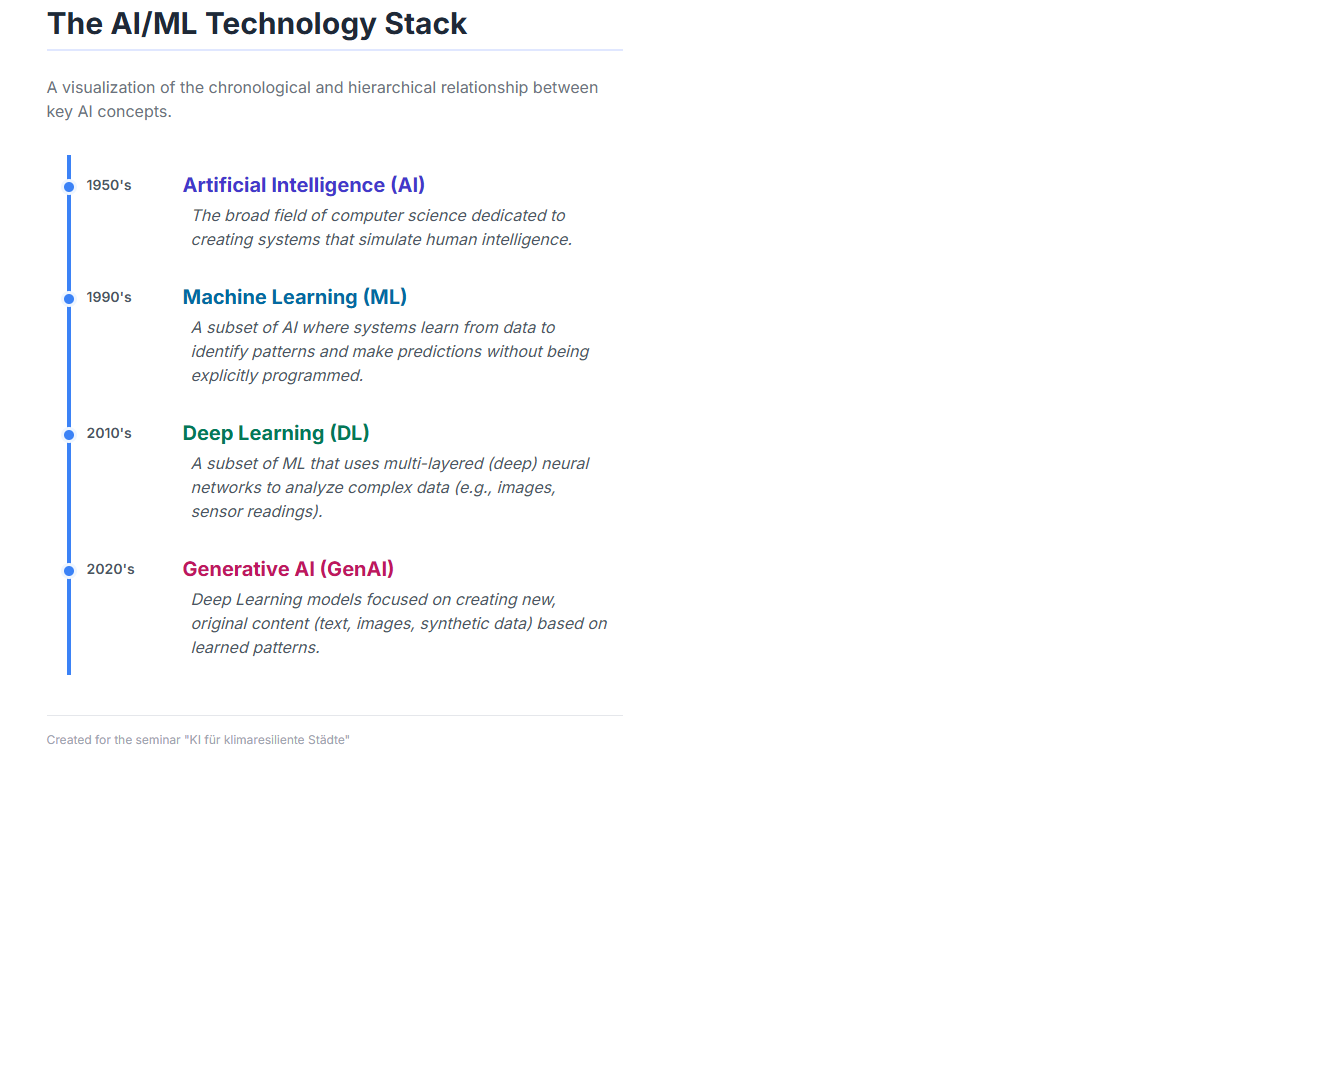
\includegraphics[width=1\textwidth]{history_AI_1.png}
    \caption{chronological evolution of AI and ML}
    \label{fig:history_AI}
\end{figure}

\subsection{Focus, Objectives, and Scope}

This seminar paper investigates the transformative potential of Artificial Intelligence (AI), with an 
emphasis on Machine Learning (ML) techniques, to create climate-resilient cities (Smart Cities). The analysis is 
structured around two specific, interconnected applications, forming the scope of this work:
\begin{itemize}
    \item \textbf{AI-Driven Prediction:} The use of ML models, integrating remote sensing (satellite data) and dense sensor networks,
to provide highly accurate, localized, and timely forecasts for key risks such as heatwaves (Hitzewellen) and heavy 
rainfall (Starkregen).

    \item \textbf{Infrastructure Optimization:} The application of AI for the dynamic, real-time control of urban systems, focusing
specifically on rainwater management (e.g., in the context of the "Sponge City" concept) to maximize flood protection
and water conservation.
\end{itemize} 
Through a text-driven analysis of current research, case studies, and expert insights, this work evaluates how these 
robust and adaptive AI systems can significantly enhance urban resilience and outlines the necessary social, economic, 
and technical conditions for their sustainable implementation.
\section{Materials and Methods}
\lipsum[4-5]\cite{ref01}  % Subsection with more details

\section{Results}
\lipsum[6-7]\cite{ref02}  % Results section

\section{Discussion}
\lipsum[8-9]\cite{ref03}  % Discussion of the results

\section{Bibliography}
\printbibliography[heading=none]


\section{Appendix}
\lipsum[10]

\end{document}
